%\section{Data}

\subsection{Imaging dataset}
%\item intro to M83: global parameters (distance, size, environment)
The dataset used for this study is the Wide-Field Camera-3
Early Release Science (ERS) observations of the nearby spiral galaxy Messier 83 (M83).
M83 is a grand-design spiral of type SAB, located at a distance of 4.66~Mpc \citep{tully13}
and the largest member of the M83 subgroup of the nearby Centaurus group of galaxies \citep{tully15}.
The galaxy's apparent radius of $\sim12$~arcmin \citep{} is reasonably well-matched to the camera's field of view (XX true? XX)
{\bf And here we note some other interesting things about M83.}

%\item Intro to WFC3 ERS dataset
%\item existing studies with this dataset (cluster, massive stars, etc)
% ref: chandar10, section. TODO: check for (unintentional!) plagiarism
The objective of the ERS observations as a whole was to probe star formation in galaxies.
The observations of M83 were made in broad- and narrow-band filters in order to characterize both stellar and nebular properties.
They cover a $3.6\times3.6$~kpc$^2$ region in the northern portion of the galaxy, including the nucleus,
a portion of a spiral arm and an interarm region.
The spatial resolution of the images is $0\farcs0396$~arcsec~pixel$^{-1}$,
corresponding to a linear scale of $XX$~pc~pixel$^{-1}$ at the 4.66~Mpc distance.
A complete description of the observations and data processing is given by \citet{chandar10};
our work here uses the observations in the UVIS channel, listed in Table~\ref{tab:filters}.
A number of previous studies have used the ERS M83 dataset for various purposes.
These include studies of 
star clusters \citep{chandar10, wofford11, whitmore11, bastian11, bastian12, fouesneau12, silva13, andrews14, chandar14, adamo15,ryon15,hollyhead15, sun16},
H~{\sc ii} regions \citep{liu13}, supernova remnants and the interstellar medium \citep{dopita10, hong11, blair14, blair15}, 
resolved stars \citep{kim12, williams15},
and a super-Eddington off-nuclear black hole \citep{soria14}.


\begin{table}
\centering
\caption{
\label{tab:filters}}
\begin{tabular}{lll}
\hline\hline
Filter & Name & Exposure time\\
\hline
F225W &  Wide UV & 1800~s\\
F336W &  $U$-band & 1890~s\\ 
%F373N &  [\ion{O}{iii}] & 2400~s\\
F438W &  $B$-band & 1180~s\\
F487N &  H$\beta$ & 2700~s\\
%F502N &  [\ion{O}{ii}] & 2484~s
F555W &  V-band, South field & 1203~s\\
%F547M &  V-band, North field & \\
%F657N &  H$\alpha$+[\ion{N}{ii}]& 1484~s\\ 
%F673N &  [\ion{S}{ii}] & 1850~s\\
F814W &  $I$-band & 1203~s\\
\hline
\end{tabular}
\end{table}

We analyze the catalog produced by \citet{chandar10} and made available via **REF**, hereafter referred to as the `ERS catalog.'
The objects in this catalog were detected on a `white-light' image produced by a weighted combination of the $UBVI$ images.
Photometry in 0.5- and 3-pixel radius apertures at the positions of the detected sources was performed on the broad- and narrow-band images and tabulated in the Vega magnitude system. 
We apply the correction to the F657N magnitude zeropoint (from 20.72 to 22.35) noted in the header of the catalog.
\citet{chandar10} discussed aperture corrections for this catalog, but since we are primarily concerned with colours
and the aperture correction does not vary strongly with wavelength, we omit it.
The catalog contains about 68000 objects which are expected to include individual stars, star clusters, stellar blends,
supernova remnants, H${\sc ii}$ regions, planetary nebulae, and background galaxies.
%TODO: foreground stars?
Completeness and reliability of the catalog are not discussed by \citet{chandar10},
but a visual inspection of the the detected sources on the white-light image suggests that a reasonable balance
between completeness and reliability was achieved.
Nine objects are flagged in the catalog as being problematic 
and we remove them from our analysis.

[to be re-organized] As a check on the catalog we used Sextractor to detect and photometer objects in the individual images.
While the aperture photometry measurements matched well, the derived uncertainties were much smaller than those reported in the catalog.
Indeed, the catalog uncertainties seem to be physically unreasonable, with median uncertainty values well above 1~magnitude in
most bandpasses, and the catalog notes do not recommend them for use except in a relative sense.
Our comparison implied that recovering a more typical magnitude uncertainty distribution would be accomplished by
dividing the 0.5-pixel magnitude uncertainties  by 10 for the broad-band filters and 15 for the narrow-band filters.
This allows us to use the catalog aperture magnitudes as an indicator of detected signal-to-noise: our analysis uses only objects with
(scaled) 0.5-pixel magnitude uncertainties $<0.2$~mag.
For the remainder of the analysis we use magnitudes measured in the 0.5-pixel radius aperture, as these should be less affected
by crowding and the variable galaxy background.

Table~\ref{tab:cat_numbers} and Figure~\ref{fig:mag_unc} characterize the catalog in terms of measurements in individual filters.
Not all objects are detected in all filters;
Table~\ref{tab:cat_numbers} gives the number of objects for which photometry is reported in a given filter,
the number for which scaled 0.5-pixel magnitude uncertainty is $0.2$~mag or less,
and the aperture magnitude at which the median magnitude uncertainty is $0.2$~mag. % Discuss last column and why 555 - should be because it is the broad filter with the most detections used for the whitelight image?
Figure~\ref{fig:mag_unc} shows the distributions of magnitudes and uncertainties in a broad and narrow filter. % See appendix for complete list of figures

%AK: please calculate numbers here. For the last column scipy.stats.binned_statistic is a good way to do this.
%Numbers are calculated based on the 0.5 aperture filters - can be changed if we decide otherwise
\begin{table}
\centering
\caption{
\label{tab:cat_numbers}}
\begin{tabular}{lrrlr}
\hline\hline
Filter & $N_{\rm obj}$ & $N_{\rm good}$ & $m_{\rm good}$ & $N_{\rm X-555}$\\
\hline
F225W &  57237 & 15011 & m & 14976\\
F336W &  62192 & 34129 & m & 33692\\
F373N &  55966 & 8878 & m & 8853\\
F438W &  66356 & 48858 & m & 48660\\
F487N &  63812 & 13335 & m & 13322\\
F502N &  64313 & 14654 & m & 14644\\
F555W &  67424 & 65652 & m & $-$\\
F657N &  67782 & 67634 & m & 65502\\
F673N &  65305 & 25295 & m & 65502\\
F814W &  67050 & 59600 & m & 57935\\
\hline
\end{tabular}
\end{table}

%AK: here's where the plots go.
\begin{figure*}
\centering
\subfloat[Broad filter distribution.]{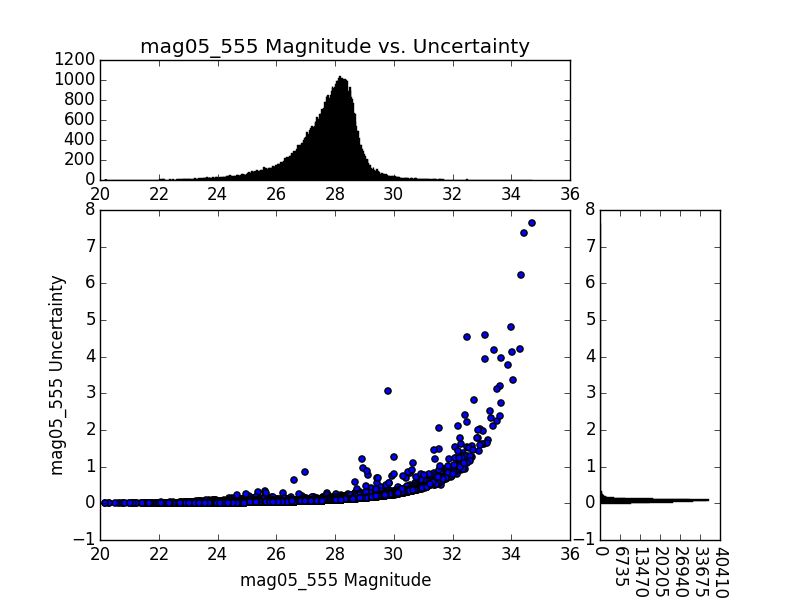
\includegraphics[width=0.5\textwidth]{figs/mag05_555_uncertainty_distribution}\label{fig:mag_unc_broad}}
\hfill
\subfloat[Narrow filter distribution.]{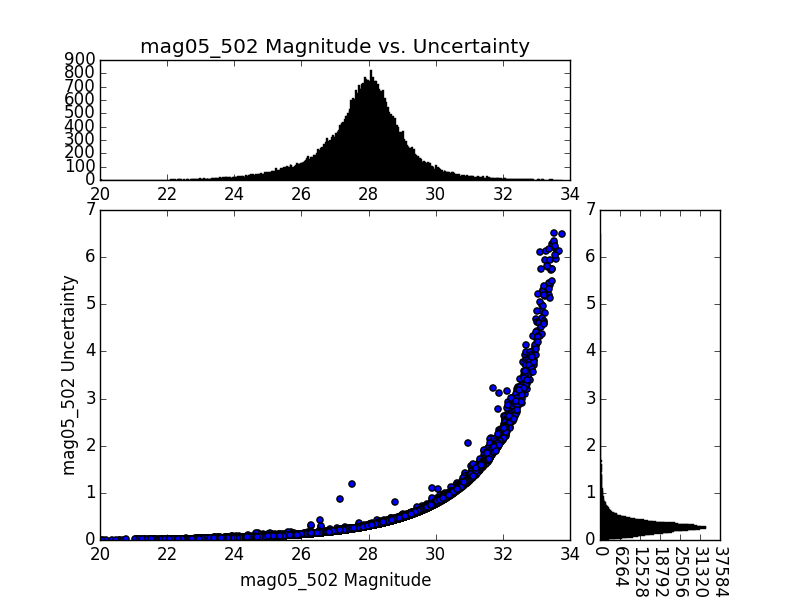
\includegraphics[width=0.5\textwidth]{figs/mag05_502_uncertainty_distribution}\label{fig:mag_unc_narrow}}
\caption{Distribution of magnitudes and uncertainties for objects in the \citet{chandar10} M83 ERS catalog.}
\label{fig:mag_unc}
\end{figure*}

% TODO: discuss (this might also go in a different section)
Our analysis in this paper is primarily concerned with colours, rather than luminosities.
Uncertainties in colours are computed as the quadrature sum of the relevant magnitudes.
Observations in 10 bands allow the generation of 45 different colours,
but not all of these colours are likely to be useful in characterizing components of the galaxy.
As the F555W band has the most individual detections, %TODO: AK: is this true?
we initially compute colours relative to this band.
The last column of Table~\ref{tab:cat_numbers} gives the number of objects for which a `good' colour (uncertainty $<0.2$~mag) is available.
%TODO: may use different number than 0.2.

\subsection{Published catalogs}

As one check on the results of our analysis, we use previously-published identifications of specific types of objects in M83.
We compiled a `published catalog' by combining the contents of the NASA Extragalactic Database (NED) and
[what does it stand for?] \citep[SIMBAD][]{wenger2000} and then adding the catalogs of Wolf-Rayet stars \citep{kim12} and
red supergiant candidates \citep{williams15}, which did not appear in either database.
NED's focus as an extragalactic database and SIMBAD's focus on Galactic objects mean that their contents overlap but are not identical, 
and this is true of the area surrounding M83. A $3\farcm3$ radius region around the coordinates centered at  ($204.26761\deg, -29.839939\deg$)
contains 1553 NED objects and 1772 SIMBAD objects, of which 1220 are matched with each other at 1\arcsec tolerance.
Although the two services use slightly different naming conventions, with human inspection the matches are generally recognizable as referring
to the same object. Interestingly, the databases do not always report the same object type even when the names are identical.
The differences are reasonable in some cases (a supernova remnant can also be an X--ray source, for example), but not others
(e.g. CXOU J133703.0-294945 is reported as a supernova remnant by SIMBAD and an H${\sc ii}$  region by NED).
A detailed study of the databases is beyond the scope of this work; for the purposes of this analysis, we kept the NED classification
for objects which appeared in both databases.
Objects which appeared in one database but not the other were primarily from recent work \citep[e.g.][]{long2014}, from
older studies likely superseded by newer ones \citep[e.g.][]{larsen1999}, or from studies in which only coordinates relative to
the galaxy centre were given \citep{rumstay83,dvpd83}.

Our final combined catalog has 2425 objects of which 750**check** are in the region covered by the ERS catalog.
The main classes are star clusters (350), X--ray sources (105), supernova remnants (86), H${\sc ii}$ regions (81),  and
radio sources (36).
Nearly every entry in the published catalog had an ERS catalog object within 1\arcsec, and the mean distance between
matched objects was 0\farcs26.
Given the nearly 100-fold difference in object density between the two catalogs, matching based on positions alone may 
result in spurious matches **REF**. *Some discussion of the exact matching procedure is warranted here, and a conclusion
on what the best thing to do is.**


%Outline for data section
%%\begin{enumerate}
%\item Intro to WFC3 ERS dataset
%\item intro to M83: global parameters (distance, size, environment)
%\item existing studies with this dataset (cluster, massive stars, etc)
%\item description of catalog (is there a ref for this??)
%\item anything about these data we don't like/didn't use?

%\end{enumerate}

